% !TEX root = catron-dissertation.tex
\epstopdfsetup{outdir=./images/05_synthetic_wavefront/}

\chapter{Synthetic Wavefront}
In order to best understand how some basic filters preform on a set of data, a fully known synthetic wavefront was generated such that all of the various components could be generated separately with the combined product filtered and compared to the synthetic wavefront containing only relevant aero-optical data.
This is done by creating an input dispersion plot where each source component is separately generated with parameters that can be modified to alter the output signal as necessary.
Signals that are assumed to be statistically independent are converted into dimensional space separately and then summed together.
While signals that are assumed to be related to one another (such as the sound and vibration components) are summed together in frequency space.
Figure \ref{fig:05_synthetic_dispersion_input} shows the input dispersion plot with each signal component separately colored.
\begin{figure}
 \centering
 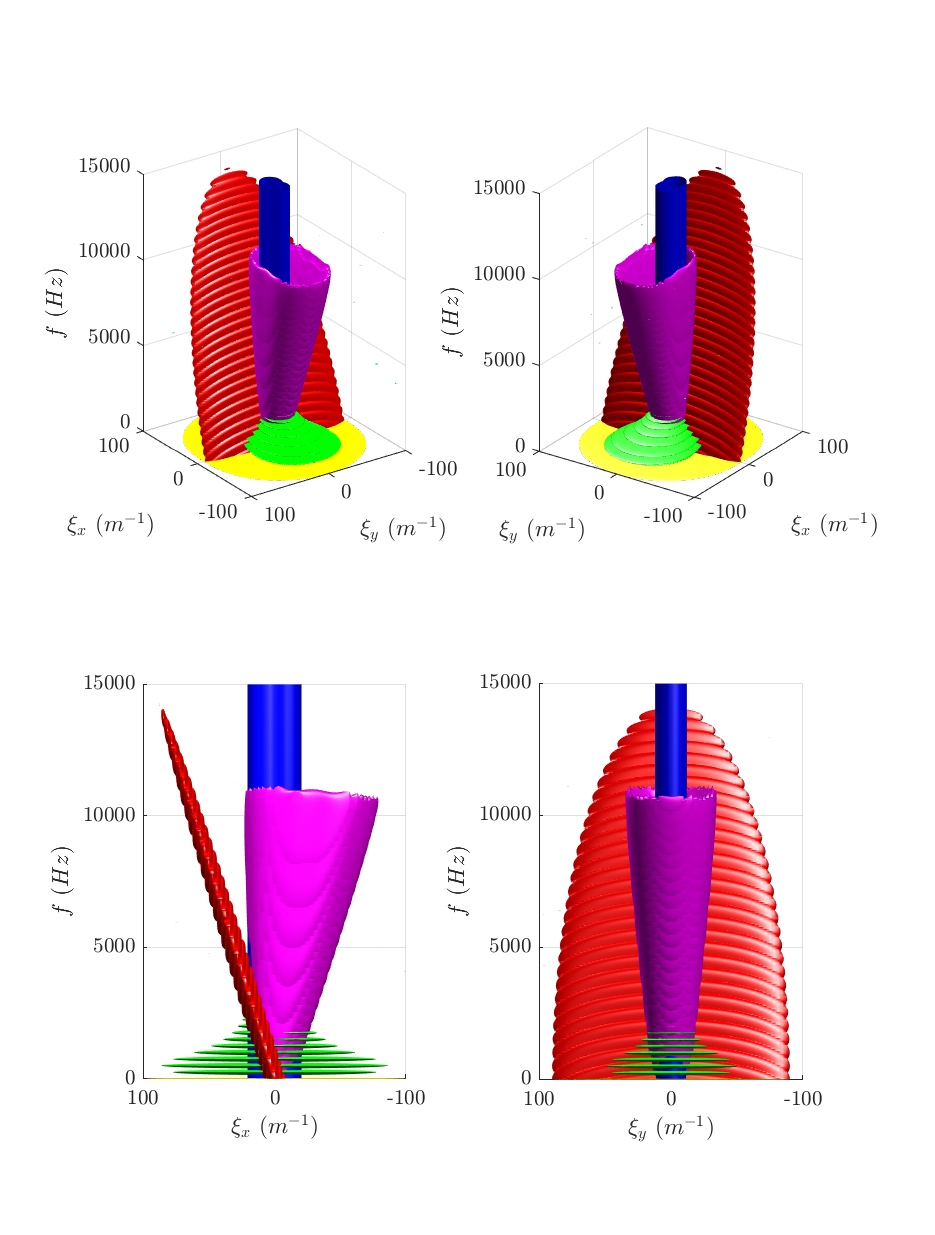
\includegraphics{../matlab/05_synthetic_wavefront/synthetic_wavefront.eps}
 \caption{Synthetic wavefront input dispersion plot of an aero-optical signal and various signal corruption components.  The aero-optical signal is shown in red, the stationary modes in blue, duct acoustics in magenta, blade-passing frequency related corruption in green, slowly varying mean-lensing in yellow, and background in cyan.}
 \label{fig:05_synthetic_dispersion_input}
\end{figure}
The aero-optical signal is shown in red, the stationary modes in blue, duct acoustics in magenta, blade-passing frequency related corruption in green, slowly varying mean-lensing in yellow, and background in cyan.

Wavefronts were generated to approximate the sample conditions in that the data presented in Figure \ref{fig:04_dispersion_3d} were measured with.
The sample rate was 200 m$^{-1}$ with 64 ($2^6$) samples in the spatial dimensions and 30,000 Hz with 8192 ($2^{13}$) samples in the temporal dimension.
The speed of sound was chosen to be 340 m/s, with a Mach number of 0.6, and a boundary layer velocity of 163.2 m/s ($0.8U_\infty$).

The general process of developing most of the component signals was to determine an approximate shape, normalize it in the appropriate dimensions, and scale the result by using a function derived from a hyperbola,
\begin{equation}
 \frac{\log_{10}(WF)-b}{b^2}-\frac{\xi_{\rho_N}^2}{a^2} = 1 \textrm{,}
 \label{eqn:05_scaling_hyperbola}
\end{equation}
such that the signal strength at unity of the normalized radial frequency, $\log_{10}(WF(\xi_{\rho_N}=1))$, and the limiting slope, $a/b$, are inputs.
This results in the signal strength of the wavefront being
\begin{equation}
 \log_{10}(WF) = b-\sqrt{\frac{\xi_{\rho_N}^2}{m^2}+b^2} \textrm{,}
 \label{eqn:05_wavefront_strength}
\end{equation}
where
\begin{equation}
 b = \frac{1}{2\log_{10}(WF(\xi_{\rho_N}=1))}\cdot\left(\log_{10}(WF(\xi_{\rho_N}=1))^2-\frac{1}{m^2}\right) \textrm{.}
 \label{eqn:05_wavefront_strength_b}
\end{equation}
The code used to generate the synthetic wavefront used in this section is shown in Listing \ref{code:sc_synthetic_wavefront}.

\section{Aero-Optical Signal}
The aero-optical signal which is approximating an optical beam passing through a boundary layers normal to each of the test section walls.
This signal was approximated by creating an ellipsoid in the plane of the feature's velocity and normalizing the radius by some arbitrary factors to roughly match the shape of the measured dispersion plot shown in Figure \ref{fig:04_dispersion_3d}.
The dispersion magnitude was then calculated by applying Equation \ref{eqn:05_wavefront_strength}, with relevant code shown on Lines 19-30 of Listing \ref{code:sc_synthetic_wavefront}.
In Figure \ref{fig:05_synthetic_dispersion_input} the aero-optical signal is shown in red.

\section{Stationary Mode Signals}
The stationary modes in Figure \ref{fig:04_dispersion_3d} appear to be temporally white-noise with the spatial frequencies forming an epicycloid of $k=2$.
This shape was further simplified using a single trigonometric function to represent the normalization function of the radial spatial frequency,
\begin{equation}
 \xi_{\rho_N} = \frac{\xi_\rho}{\xi_{\rho_0}\sqrt{10-6\cos{(2\xi_\theta)}}} \textrm{,}
\end{equation}
this makes an epicycloidal like shape which has a smooth derivative.
This dispersion component is shown in blue in Figure \ref{fig:05_synthetic_dispersion_input} and the relevant code shown in Lines 61-66 of Listing \ref{code:sc_synthetic_wavefront}.

\section{Sound \& Vibration Signals}
The sound \& vibrating component signals are comprised of two parts.
The first of these is the blade-passing frequency and its harmonic disturbances (shown in green in Figure \ref{fig:05_synthetic_dispersion_input}) and the second is the acoustic duct modes (shown in magenta).
Like the stationary modes, the blade-passing frequency disturbances were modeled with the simplified epicycloid narrow-band disc and each harmonic was modulated by using a low-pass filter offset to the blade-passing frequency.
The code for the blade-passing frequency disturbances is shown in Lines 97-113 of Listing \ref{code:sc_synthetic_wavefront}.

The acoustic duct mode disturbances form a cone which in the $f-\xi_x$ plane is defined by the lines $u\pm c$, while in the $f-\xi_y$ plane is defined by the speed of sound.
At each temporal frequency step an ellipse was defined based on the constraining lines and the distance to that ellipse used to calculate a normalized radial frequency.
The strength of the disturbance was decreased logarithmically in temporal frequency as shown in the code in Lines 183-200 of Listing \ref{code:sc_synthetic_wavefront}.

\section{Mean Lensing Signal}
The mean-lensing signal (shown in yellow in Figure \ref{fig:05_synthetic_dispersion_input}) uses a stretched version of the simplified epicycloid and represents the slowly varying spatial disturbance.
The relevant code is shown on Lines 144-152 of Listing \ref{code:sc_synthetic_wavefront}.

\section{Background Noise Signal}
The background noise disturbance (with a few small spots shown in cyan in Figure \ref{fig:05_synthetic_dispersion_input}) was the only component that did not use the hyperbola to scale the signal but instead was just normally distributed random noise with a mean noise level and deviation as inputs.
The relevant code is shown in Lines 230-234 of Listing \ref{code:sc_synthetic_wavefront}.

\section{Synthetic Wavefront Creation}
A synthetic signal can be created from a power spectra by solving for $x$ in Equation \ref{eqn:05_basic_sxx} and using the Inverse Fast Fourier Transform,
\begin{equation}
 x(t) = \real\left[\ifft\left\{\sqrt{S_{xx}\cdot N\cdot f_{samp}}\cdot\exp{i\phi}\right\}\right] \textrm{,}
 \label{eqn:05_ifft}
\end{equation}
where $\real$ is the real component and $\phi$ is a random set of phases for each point in the measurement space.
As shown previously this relation can be extended into $n$-dimensions,
\begin{equation}
 f(\mathbf{x}) = \real\left[\ifftn\left\{\sqrt{\mathbf{S_{xx}}\cdot\prod{\overrightarrow{N}\cdot \overrightarrow{f}_{samp}}}\cdot\exp{i\mathbf{\phi}}\right\}\right] \textrm{.}
 \label{eqn:05_ifftn}
\end{equation}
Care should be taken when constructing the random set of phases, as the zero-frequency component has zero phase and the phases on either side of it are conjugates of one another.
The code for creating a wavefront from a dispersion plot is shown in Lines 336-340 of Listing \ref{code:sc_synthetic_wavefront} and is specifically creating the wavefront for the aero-optical signal but other signals are generated using the same basic code.
Note that the first three lines are to get the set of phases properly configured that creates conjugate phases rotated about the origin.

It was assumed that the aero-optical signal, the stationary modes, and the background noise were statistically independent of one another and the sound and vibration combination of modes and as such could be separately transformed into physical space.
While the components of the sound and vibration sources, the blade-passing frequency, the acoustic cone, and the mean-lensing, were assumed to be related to one another and thus were summed together in frequency space prior to being transformed into physical space.
Once the separate components were in physical space the total wavefront was obtained by summing up the separate components with the aero-optical signal being a separately saved along side the total wavefront.
Some frames from the synthetic wavefront are shown in Figure \ref{fig:05_synthetic_frames} with the total wavefront shown on top and the aero-optical only signal shown on the bottom.
\begin{figure}
 \centering
 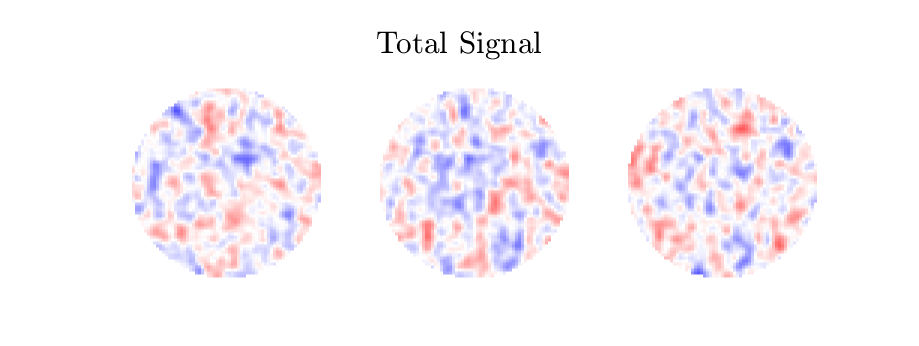
\includegraphics{../matlab/05_synthetic_wavefront/synthetic_frames_total.eps}
 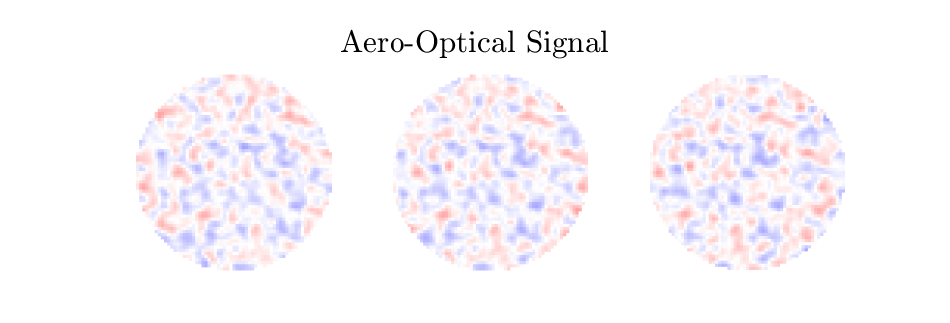
\includegraphics{../matlab/05_synthetic_wavefront/synthetic_frames_ao.eps}
 \caption{Sample frames from the synthetic wavefront with the total wavefront signal on top and the aero-optical only signal bottom.  Flow is from right to left.}
 \label{fig:05_synthetic_frames}
\end{figure}
Flow is from right to left.
The aero-optical signal is often times noticeable in the total wavefront signal, but can be easily overpowered by the various contamination sources.

\section{Comparison to Measured Data}
A dispersion plot of the total synthetic wavefront is shown in Figure \ref{fig:05_dispersion_synthetic}.
\begin{figure}
 \centering
 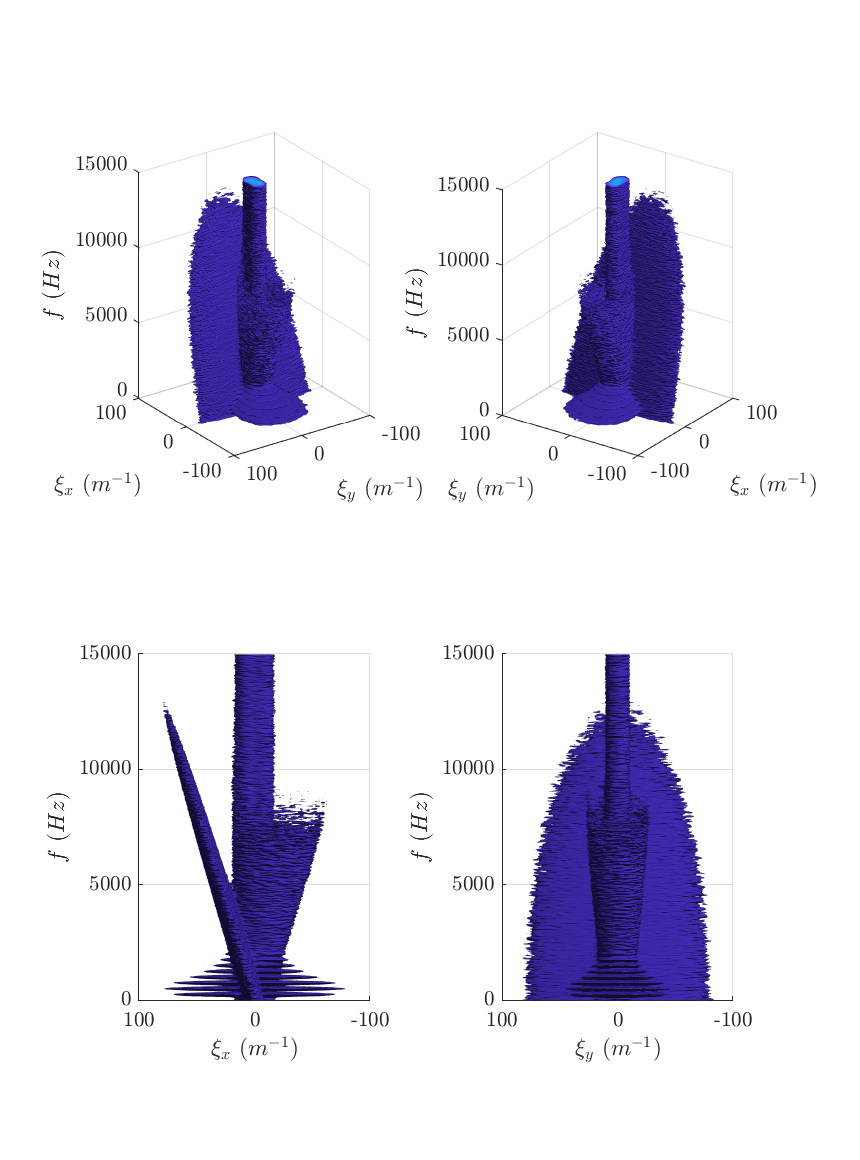
\includegraphics{../matlab/05_synthetic_wavefront/dispersion_synthetic.eps}
 \caption{Synthetic wavefront output dispersion plot of an aero-optical signal and various signal corruption components.}
 \label{fig:05_dispersion_synthetic}
\end{figure}
In this view the aero-optical signal is more noticeable but there still remains some significant overlap with the various contamination sources.
While the mean-lensing component is not as visible in this isosurface, the rest of the dispersion plot in a good representation of the input dispersion plot shown in Figure \ref{fig:05_synthetic_dispersion_input}.
The blade-passing frequency was depicted as symmetric in the synthetic wavefront while measured data (shown in Figure \ref{fig:04_dispersion_3d}) shows more signal on the side traveling in the direction of flow.
The harmonics of the BPF are more on the upstream traveling side of the dispersion and are a little less pronounced in the measured data.
The total synthetic wavefront has a spatial time-averaged RMS of $0.0112\pm0.0006\mu m$ with the aero-optical only signal having a spatial time-averaged RMS of $0.0073\pm0.0003\mu m$.
The measured wavefront presented in Figure \ref{fig:04_dispersion_3d} had a spatial time-averaged RMS of $0.0874\pm0.0263\mu m$.
The overall spatial RMS of the synthetic wavefront was $12.8\%$ when compared to the measured wavefront indicating that the algorithms used to generate the wavefront are not representative of reality and can provide a future path of research in order to produce more realistic synthetic wavefronts.
\textcolor{red}{Double Check line numbers for the Listings.}
